\documentclass{beamer}

\usepackage{emoji}
\usepackage{pgfplots}

\usetheme{UiO}

\title{SMBers rolle i å fylle implementeringsgapet innen AI og helse}
\author{Esten H. Leonardsen}
\date{06.03.2024}

\titlegraphic{
	\centering
	\vspace{7.7cm}
	
\includegraphics[width=\logowidth]{data/uio_logo_full.png}
}

\usetikzlibrary{arrows}
\usetikzlibrary{arrows.meta}
\usetikzlibrary{calc}
\usetikzlibrary{fadings}
\usetikzlibrary{fillbetween}
\usetikzlibrary{patterns}
\usetikzlibrary{positioning}
\usetikzlibrary{shapes.arrows}

\begin{document}
	\begin{frame}
	 	\titlepage
	\end{frame}

    \newcommand{\stickman}[2]{
        \node[circle,fill,minimum size=2.5mm,#2] (head) at #1 {};
        \node[rounded corners=1pt,minimum height=0.65cm,minimum width=0.2cm,fill,below = 0.5pt of head,#2] (body) {};
        \draw[line width=0.5mm,round cap-round cap,#2] ([shift={(1pt,-0.5pt)}]body.north east) --++(-90:3mm);
        \draw[line width=0.5mm,round cap-round cap,#2] ([shift={(-1pt,-0.5pt)}]body.north west)--++(-90:3mm);
        \draw[thick,white,-round cap] (body.south) --++(90:2.75mm);
    }


    \newcommand{\population}{
        \begin{tikzpicture}
            \node [
                double arrow,
                left color=blue,
                right color=red,
                double arrow head extend=0pt,
                transform shape,
                minimum height=1.5cm,
                text width=2.6cm,
                anchor=west
            ] at (-0.5, -1.25){};
            \node[font=\tiny, text=white] at (1.08, -1.25) {Symptomnivå};
            \stickman{(0, 0)}{blue}
            \stickman{(0.5, -0.1)}{blue}
            \stickman{(0.1, 1.1)}{blue}
            \stickman{(0.7, 1.05)}{blue}
            \stickman{(1.15, 0.1)}{blue}
            \stickman{(1.8, 0.2)}{blue!50!red}
            \stickman{(0.4, 2.2)}{blue!80!red}
            \stickman{(1.3, 1.4)}{blue!60!red}
            \stickman{(1.8, 2.2)}{blue!20!red}
            \stickman{(2.3, 1.2)}{blue!10!red}
        \end{tikzpicture}
    }

    % \newcommand{\mriside}[5]{
    %     \node[inner sep=0pt] (input) at (#1, #2) {
    %         \includegraphics[height=#3, width=#3]{#4}
    %     };

    %     \draw[fill=black] (input.north west) --
    %         ($ (input.north west) + (0.5 * #5, 0.5 * #5) $) --
    %         ($ (input.north east) + (0.5 * #5, 0.5 * #5) $) --
    %         (input.north east) -- cycle;
    %     \draw[fill=black] (input.north east) --
    %         ($ (input.north east) + (0.5 * #5, 0.5 * #5) $) --
    %         ($ (input.south east) + (0.5 * #5, 0.5 * #5) $) --
    %         (input.south east) -- cycle;
    %     \draw[] (input.north west) --
    %         ($ (input.north west) - (0.5 * #5, 0.5 * #5) $) --
    %         ($ (input.south west) - (0.5 * #5, 0.5 * #5) $) --
    %         (input.south west) -- cycle;
    %     \draw[] (input.north east) --
    %         ($ (input.north east) - (0.5 * #5, 0.5 * #5) $) --
    %         ($ (input.south east) - (0.5 * #5, 0.5 * #5) $) --
    %         (input.south east) -- cycle;
    %     \draw[] ($ (input.north west) - (0.5 * #5, 0.5 * #5) $) --
    %         ($ (input.north east) - (0.5 * #5, 0.5 * #5) $);
    %     \draw[] ($ (input.south west) - (0.5 * #5, 0.5 * #5) $) --
    %         ($ (input.south east) - (0.5 * #5, 0.5 * #5) $);
    % }


    % \newcommand{\inputside}[4]{
    %     \mriside{#1}{#2}{#3}{data/mri_sagittal.png}{#4}
    % }
    % \newcommand{\heatmapside}[3]{
    %     \mriside{#1}{#2}{#3}{data/combined_sagittal.png}
    % }
    % \newcommand{\convside}[6]{
    %     \def\sidex{#1}
    %     \def\sidey{#2}
    %     \def\sidewidth{#3}
    %     \def\sideheight{#4}
    %     \def\sidefillcolour{#5}
    %     \def\sidename{#6}

    %     \node[
    %         fill=\sidefillcolour,
    %         inner sep=0pt,
    %         outer sep=0pt,
    %         minimum width=\sidewidth,
    %         minimum height=\sideheight,
    %         draw=black
    %     ] (\sidename) at (\sidex, \sidey) {};
    % }

    % \newcommand{\convtop}[4]{
    %     \def\topbase{#1}
    %     \def\topwidth{#2}
    %     \def\topheight{#3}
    %     \def\topfillcolour{#4}

    %     \draw[fill=\topfillcolour,draw=black] #1 --
    %         ($ #1 + (#3, #3) $) --
    %         ($ #1 + (#3+#2, #3) $) --
    %         ($ #1 + (#2, 0) $);
    % }

    % \newcommand{\convfront}[3]{
    %     \def\frontbase{#1}
    %     \def\frontsize{#2}
    %     \def\frontfillcolour{#3}

    %     \draw[black, fill=\frontfillcolour] #1 --
    %         ($ #1 + (1*#2, 1*#2) $) --
    %         ($ #1 + (1*#2, 1*#2 - 2*#2) $) --
    %         ($ #1 + (0, -2*#2) $);
    % }

    % \newcommand{\convchannel}[7]{
    %     \def\channelx{#1}
    %     \def\channely{#2}
    %     \def\channelnodedepth{#3}
    %     \def\channelnodesize{#4}
    %     \def\channelnodecount{#5}
    %     \def\channelcolour{#6}
    %     \def\includefront{#7}

    %     \def\huemin{20}
    %     \def\huemax{80}

    %     \pgfmathsetmacro{\iterations}{#5-1}
    %     \foreach \i in {0,...,\iterations} {
    %         \pgfmathsetmacro{\hue}{int(random(\huemin, \huemax))}
    %         \convside{#1}{#2+\i*-#4}{#3 cm}{#4 cm}{#6!\hue}{n\i0}

    %         \foreach \j in {0,...,\iterations} {
    %             \pgfmathsetmacro{\innerhue}{int(random(\huemin, \huemax))}
    %             \ifnum\j=0
    %                 \pgfmathsetmacro{\innerhue}{\hue}
    %             \fi

    %             \ifnum\includefront=1
    %                 \convfront{($ (n00.north east) + (0.5*\j*#4, 0.5*\j*#4 - \i*#4) $)}{0.5*#4}{#6!\innerhue}
    %             \fi

    %             \ifnum\i=0
    %                 \convtop{($ (n\i0.north west) + (0.5*\j*#4, 0.5*\j*#4) $)}{#3}{0.5*#4}{#6!\innerhue}
    %             \fi
    %         }
    %     }
    % }


    % \newcommand{\lrpchannel}[6]{
    %     \def\channelx{#1}
    %     \def\channely{#2}
    %     \def\channelnodedepth{#3}
    %     \def\channelnodesize{#4}
    %     \def\channelnodecount{#5}
    %     \def\includefront{#6}

    %     \colorlet{bgcolour}{black!85}

    %     \pgfmathsetmacro{\iterations}{#5-1}
    %     \foreach \i in {0,...,\iterations} {
    %         \pgfmathsetmacro{\hue}{int(random(-150, 100))}
    %         \colorlet{fillcolour}{bgcolour}

    %         \colorlet{lrpcolour}{red}
    %         \pgfmathsetmacro{\coinflip}{int(random(0, 1))}

    %         \ifnum\coinflip=1
    %             \colorlet{lrpcolour}{blue}
    %         \fi

    %         \ifnum\hue>0
    %             \colorlet{fillcolour}{lrpcolour!\hue!bgcolour}
    %         \fi

    %         \convside{#1}{#2+\i*-#4}{#3 cm}{#4 cm}{fillcolour}{n\i0}

    %         \foreach \j in {0,...,\iterations} {
    %             \pgfmathsetmacro{\innerhue}{int(random(-150, 100))}
    %             \colorlet{innerfillcolour}{bgcolour}

    %             \ifnum\innerhue>0
    %                 \colorlet{innerfillcolour}{lrpcolour!\innerhue!bgcolour}
    %             \fi

    %             \ifnum\j=0
    %                 \colorlet{innerfillcolour}{fillcolour}
    %             \fi

    %             \ifnum\includefront=1
    %                 \convfront{($ (n00.north east) + (0.5*\j*#4, 0.5*\j*#4 - \i*#4) $)}{0.5*#4}{innerfillcolour}
    %             \fi

    %             \ifnum\i=0
    %                 \convtop{($ (n\i0.north west) + (0.5*\j*#4, 0.5*\j*#4) $)}{#3}{0.5*#4}{innerfillcolour}
    %             \fi
    %         }
    %     }
    % }

    % \newcommand{\convlayer}[7]{
    %     \def\layerx{#1}
    %     \def\layery{#2}
    %     \def\layernodedepth{#3}
    %     \def\layernodesize{#4}
    %     \def\layernodecount{#5}
    %     \def\layerdepth{#6}
    %     \def\layercolour{#7}

    %     \pgfmathsetmacro{\layeriterations}{\layerdepth-1}
    %     \foreach \i in {0,...,\layeriterations}{
    %         \pgfmathsetmacro{\x}{\layerx + \i * \layernodedepth}
    %         \pgfmathsetmacro{\islast}{\i == \layeriterations ? 1 : 0}
    %         \convchannel{\x}{\layery}{\layernodedepth}{\layernodesize}{\layernodecount}{\layercolour}{\islast}
    %     }
    % }

    % \newcommand{\lrplayer}[6]{
    %     \def\layerx{#1}
    %     \def\layery{#2}
    %     \def\layernodedepth{#3}
    %     \def\layernodesize{#4}
    %     \def\layernodecount{#5}
    %     \def\layerdepth{#6}

    %     \pgfmathsetmacro{\layeriterations}{\layerdepth-1}
    %     \foreach \i in {0,...,\layeriterations}{
    %         \pgfmathsetmacro{\x}{\layerx + \i * \layernodedepth}
    %         \pgfmathsetmacro{\islast}{\i == \layeriterations ? 1 : 0}
    %         \lrpchannel{\x}{\layery}{\layernodedepth}{\layernodesize}{\layernodecount}{\islast}
    %     }
    % }

    % \newcommand{\modelarrow}[5]{
    %     \begin{scope}[transparency group, opacity=0.5]
    %         \draw[-stealth, line width=2pt, #3] #1 to [in=#4, out=#5] #2;
    %     \end{scope}
    % }

    % \newcommand{\cnnarrow}[3]{
    %     \modelarrow{#1}{#2}{#3}{180}{0}
    % }

    % \newcommand{\lrparrow}[3]{
    %     \modelarrow{#1}{#2}{#3}{0}{180}
    % }

    % \newcommand{\cnn}[6]{
    %     \def\xmin{#1}
    %     \def\ymin{#2}
    %     \def\nodedepth{#3}
    %     \def\nodesize{#4}
    %     \def\modelcolour{#5}
    %     \def\annotation{#6}

    %     \convlayer{#1 - 0.06 + 0.4}{#2 + 2.5 * #4}{#3}{#4}{12}{3}{\modelcolour}
    %     \cnnarrow{(#1 + 0.95, #2)}{(#1+2.2, #2)}{#5}

    %     \convlayer{#1 + 1.44 + 0.4}{#2 + 1.5 * #4}{#3}{#4}{8}{5}{\modelcolour}
    %     \cnnarrow{(#1 + 2.43, #2)}{(#1+3.5, #2)}{#5}

    %     \convlayer{#1 + 2.77 + 0.4}{#2 + 0.5 * #4}{#3}{#4}{4}{7}{\modelcolour}
    %     \cnnarrow{(#1 + 3.75, #2)}{(#1+5, #2)}{#5}

    %     \convlayer{#1 + 3.93 + 0.4}{#2 + 0}{#3}{#4}{2}{9}{\modelcolour}

    %     \draw[thick, dashed] (#1 + 0.22, #2 + 1.43) --
    %                         (#1 + 5.13, #2 + 1.43) --
    %                         (#1 + 5.13, #2 - 1.42) --
    %                         (#1 + 0.22, #2 - 1.42) -- cycle;
    %     \node[anchor=south, text depth=0] at (#1 + 2.675, #2 + 1.43) {
    %         \textbf{#6}
    %     };
    % }
    % \newcommand{\lrp}[5]{
    %     \def\xmin{#1}
    %     \def\ymin{#2}
    %     \def\nodedepth{#3}
    %     \def\nodesize{#4}
    %     \def\annotation{#5}

    %     \lrplayer{#1 - 0.06 + 0.4}{#2 + 2.5 * #4}{#3}{#4}{12}{3}{black}
    %     \lrparrow{(#1+2.2, #2)}{(#1 + 0.95, #2)}{black}

    %     \lrplayer{#1 + 1.44 + 0.4}{#2 + 1.5 * #4}{#3}{#4}{8}{5}{black}
    %     \lrparrow{(#1+3.5, #2)}{(#1 + 2.43, #2)}{black}

    %     \lrplayer{#1 + 2.77 + 0.4}{#2 + 0.5 * #4}{#3}{#4}{4}{7}{black}
    %     \lrparrow{(#1+5, #2)}{(#1 + 3.75, #2)}{black}

    %     \lrplayer{#1 + 3.93 + 0.4}{#2 + 0}{#3}{#4}{2}{9}{black}
    %     \draw[thick, dashed] (#1 + 0.22, #2 + 1.43) --
    %             (#1 + 5.13, #2 + 1.43) --
    %             (#1 + 5.13, #2 - 1.42) --
    %             (#1 + 0.22, #2 - 1.42) -- cycle;
    %     \node[anchor=south, text depth=0] at (#1 + 2.675, #2 + 1.43) {
    %         \textbf{#5}
    %     };
    % }

    \begin{frame}{Implementeringsgapet}
        \begin{tikzpicture}
            \node[draw=black] at (-5.25, -3.5) {};
            \node[draw=black] at (5.25, 3.5) {};

            \visible<1>{
                \node[label={[yshift=0.05cm]below:\tiny{Bilde generert av ChatGPT}}, inner sep=0pt] (brain) at (-3, 0) {
                    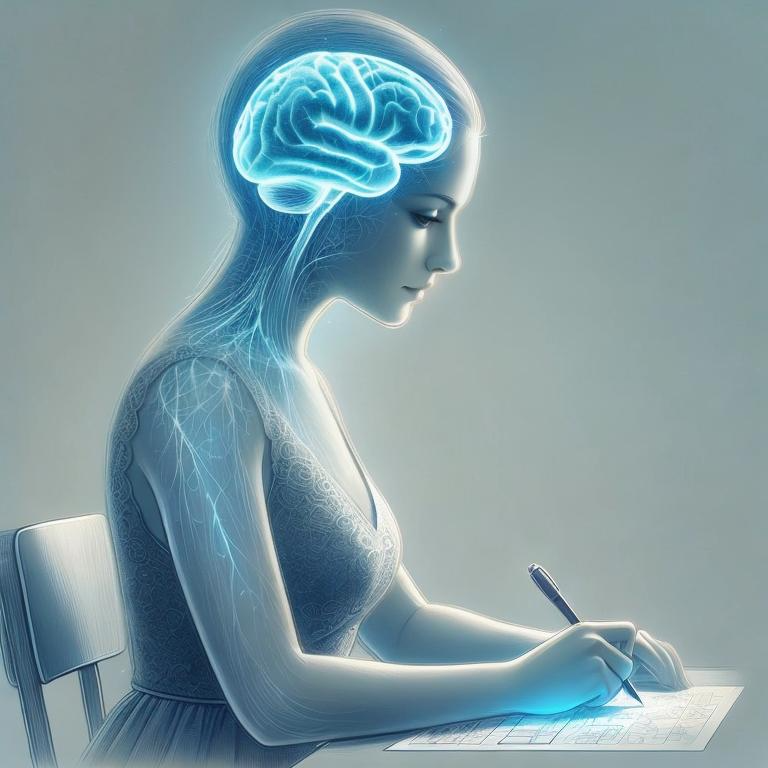
\includegraphics[width=3.5cm]{data/thinking.png}
                };
                \node[] (population) at (3, 0) {
                    \population
                };
                \draw[-stealth, line width=5pt, black!40] (brain) -- (population);
            }
            \visible<2-3>{
                \node[label={[yshift=-0.05cm]above:\footnotesize{27 år}}, inner sep=0pt] (input) at (-1.5, 2.5) {
                    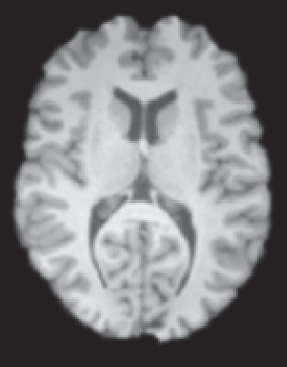
\includegraphics[height=1.5cm]{data/input.png}
                };
                \node[font=\fontsize{40}{25}] (notes) at (1.5, 2.5) {
                    \emoji{ledger}
                };
                \node[font=\tiny\linespread{0.9}\selectfont, align=center, text width=10cm, anchor=south] at (0, -3.75) {
                    Xia, T., Chartsias, A., Wang, C., Tsaftaris, S. A., \& Alzheimer’s Disease Neuroimaging Initiative. (2021). Learning to synthesise the ageing brain without longitudinal data. \textit{Medical Image Analysis}.
                };
            }
            \visible<3>{
                \node[align=center, font=\normalfont\linespread{0.9}\selectfont, draw=black, fill=teal!20, rounded corners=0.1cm, inner sep=5pt] (model) at (0, 0.5) {
                    Generativ\\kunstig intelligens
                };
                \node[label={[yshift=0.1cm]below:\footnotesize{37 år}}, inner sep=0pt] (output37) at (-2.5, -1.8) {
                    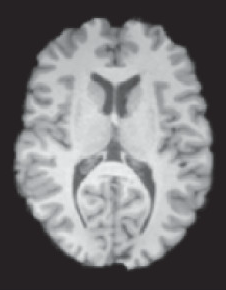
\includegraphics[height=1.5cm]{data/output_37.png}
                };
                \node[label={[yshift=0.1cm]below:\footnotesize{57 år}}, inner sep=0pt] (output57) at (0, -1.8) {
                    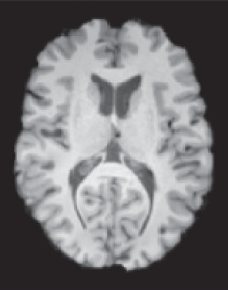
\includegraphics[height=1.5cm]{data/output_57.png}
                };
                \node[label={[yshift=0.1cm]below:\footnotesize{77 år}}, inner sep=0pt] (output77) at (2.5, -1.8) {
                    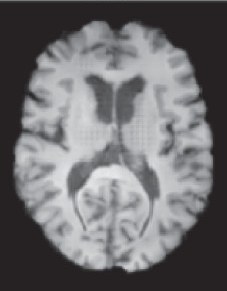
\includegraphics[height=1.5cm]{data/output_77.png}
                };

                \draw[-stealth, line width=2pt, gray] (input) to [out=270, in=90] ($ (model.north) - (0.125, 0) $);
                \draw[-stealth, line width=2pt, gray] ($ (notes.south) + (0, 0.08) $) to [out=270, in=90] ($ (model.north) + (0.125, 0) $);
                \draw[-stealth, line width=2pt, gray] (model) to [out=270, in=90] (output37);
                \draw[-stealth, line width=2pt, gray] (model) to [out=270, in=90] (output57);
                \draw[-stealth, line width=2pt, gray] (model) to [out=270, in=90] (output77);
            }
            \visible<4-8>{
                \node[font=\tiny\linespread{0.9}\selectfont, align=center, text width=10cm, anchor=south] at (0, -3.75) {
                    Leonardsen, E. H., Persson, K., Grødem, E., Dinsdale, N., Schellhorn, T., ... \& Wang, Y. (2024). Constructing personalized characterizations of structural brain aberrations in patients with dementia using explainable artificial intelligence. \textit{NPJ Digital Medicine}.
                };
            }
            % \visible<4-5>{
            %     \inputside{-4}{0}{1.5cm}{0.75}
            % }
            % \visible<5>{
            %     \cnnarrow{(input.east)}{($ (input.center) + (2, 0) $)}{blue}
            %     \cnn{-2.5}{0}{0.066}{0.15}{blue}{Kunstig nevralt nettverk}
            %     \node[align=left, font=\footnotesize\linespread{0.9}\selectfont] (output) at (4, 0) {
            %         Pasient eller\\
            %         kontroll?
            %     };
            %     \cnnarrow{($ (output.west) - (0.525, 0) $)}{($ (output.west) + (0.1, 0) $)}{blue}
            % }
            % \visible<6>{
            %     \heatmapside{-4}{0}{1.5cm}{0.75}
            %     \lrparrow{($ (input.center) + (2, 0) $)}{(input.east)}{black}
            %     \lrp{-2.5}{0}{0.066}{0.15}{Forklarbar kunstig intelligens}
            %     \node[align=left, font=\footnotesize\linespread{0.9}\selectfont] (output) at (4, 0) {
            %         Pasient eller\\
            %         kontroll?
            %     };
            %     \lrparrow{($ (output.west) + (0.1, 0) $)}{($ (output.west) - (0.525, 0) $)}{black}
            % }
            \visible<7-8>{
                \node[label=above:\small{Kunstig intelligens}, inner sep=0pt] at (-2.5, 0.5) {
                    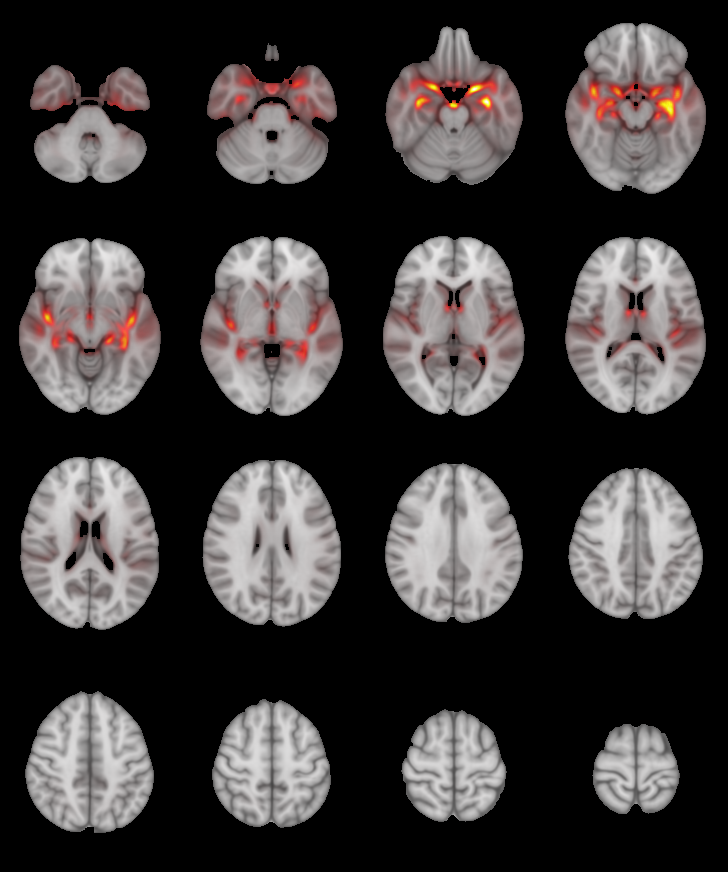
\includegraphics[width=4cm]{data/dementia_average.png}
                };
            }
            \visible<8>{
                \node[label=above:\small{Menneskelige forskere}, inner sep=0pt] at (2.5, 0.5) {
                    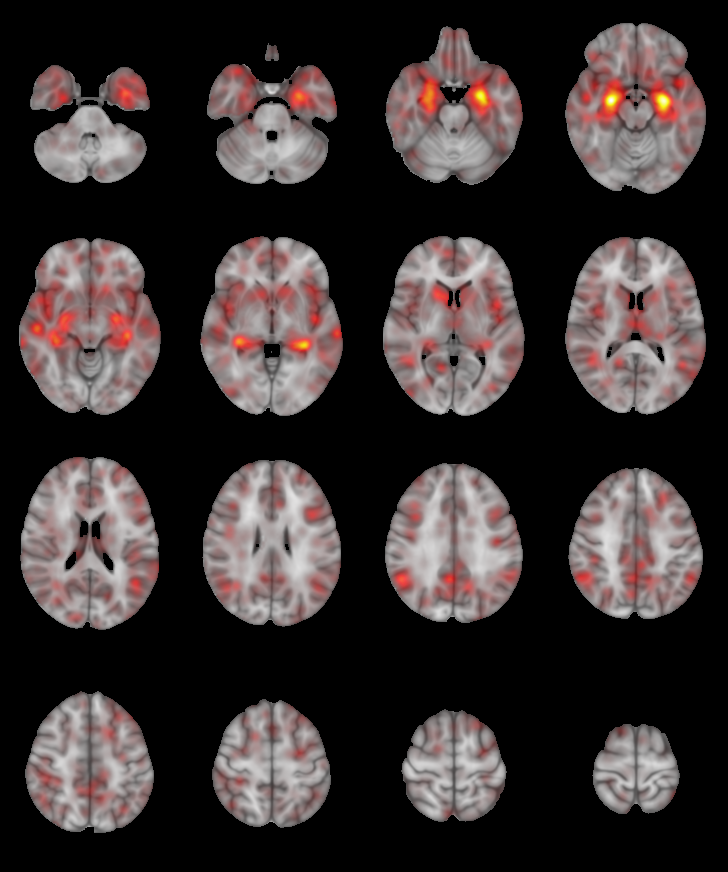
\includegraphics[width=4cm]{data/ALE.png}
                };
            }
            \visible<9-11>{
                \node[font=\tiny\linespread{0.9}\selectfont, align=center, text width=10cm, anchor=south] at (0, -3.75) {
                    Wang, Y., Gao, R., Wei, T., Johnston, L., Yuan, X., Zhang, Y., ... \& Alzheimer’s Disease Neuroimaging Initiative. (2024). Predicting long-term progression of Alzheimer’s disease using a multimodal deep learning model incorporating interaction effects. \textit{Journal of Translational Medicine}.
                };

                \node[] (imaging) at (-4, 2.5) {
                    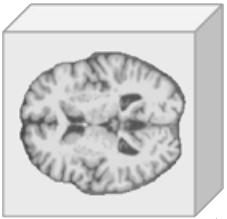
\includegraphics[height=1.5cm]{data/imaging.png}
                };
                \node[] (demographics) at (-4, 0.25) {
                    
\includegraphics[height=1.5cm]{data/demographics.png}
                };
                \node[] (genetics) at (-4, -2) {
                    
\includegraphics[height=1.5cm]{data/genetics.png}
                };
            }
            \visible<10-11>{
                \node[align=center, font=\normalfont\linespread{0.9}\selectfont, draw=black, fill=teal!20, rounded corners=0.1cm, inner sep=5pt] (model) at (0, 0.5) {
                    Multimodal\\kunstig intelligens
                };
            }
        \end{tikzpicture}
    \end{frame}

\end{document}
